TileCal is the central hadronic calorimeter of the ATLAS experiment covering the
$|\eta| < 1.7$ region. It is designed for energy measurement of hadrons, jets,
tau particles and also contributes to the measurement of missing transverse
energy (see Section~\ref{sec:miss-transv-energy}). TileCal is a scintillator
steel non compensating sampling calorimeter, the scintillation light produced in
the tiles is transmitted by wavelength shifting fibers to \glspl{pmt}. The
analog signals from the PMTs are amplified, shaped and digitized by sampling the
signal every 25~ns. The TileCal front end electronics read out the signals
produced by about 10000 channels measuring energies ranging from 30~MeV to
2~TeV. The readout system is responsible for reconstructing the data in real
time. The digitized signals are reconstructed with the Optimal Filtering
algorithm (see Section~\ref{sec:optimal-filtering}), which computes for each
channel the signal amplitude, time and quality factor at the required high rate.

TileCal is designed as one \gls{lb} and two \gls{eb}. The barrels are further
divided, according to their geometrical position on the $z$-axis, in partitions
called EBA, LBA, EBC and LBC (see Section~\ref{sec:coordinate-system}). Each
partition consists of 64 independent wedges (see Figure~\ref{fig:tile_mod})
along the azimuthal direction called \emph{modules}; the LBA and EBA partitions
are shown in Figure~\ref{fig:tile_cells}.

\begin{figure}[!h]
  \centering
    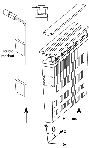
\includegraphics[width=.5\linewidth]{tile_module}
    \caption{Cut away showing the optical read out and design of a TileCal
      module.}
    \label{fig:tile_mod}
\end{figure}

Between the LB and the EB there is a 600~mm gap needed for the ID and the LAr
cables, electronics and services. Part of the gap contains the \gls{itc}, a
detector designed to maximize the active material while leaving enough space for
services and cables. The ITC is an extension of the EB and it occupies the 0.8 <
$|\eta|$ < 1.6 region. The combined 0.8 < $|\eta|$ < 1.0 part is called
\emph{plug} and in the 1.0 < $|\eta|$ < 1.6 region, for space reasons, the ITC
is not interleaved with an absorber and is only composed of scintillator
material. The scintillators between 1.0 < $|\eta|$ < 1.2 are called \emph{gap
  scintillators}, while those between 1.2 < $|\eta|$ < 1.6 are called
\emph{crack scintillators}. The plug and the gap scintillators mainly provide
hadronic shower sampling while the crack scintillator, which extends to the
region between the barrel and the end-cap cryostats, samples the electromagnetic
shower in a region where the normal sampling is impossible due to the dead
material of the cryostat walls and the ID cables.

TileCal is also divided in longitudinal layers, the A, BC and D layers as shown
in Figure~\ref{fig:tile_cells}. The two innermost layers have a
$\Delta \eta \times \Delta \phi$ segmentation of $0.1 \times 0.1$ while in the
outermost, the segmentation is $0.1 \times 0.2$. Each layer is logically divided
into \emph{cells} by grouping together in the same PMT the fibers coming from
different scintillator tiles belonging to the same radial depth. The gap/crack
scintillators are also called E layer cells.

The energy resolution for jets of ATLAS is:
\begin{equation}
  \label{eq:65}
  \frac{\sigma_E}{E} = \frac{50\%}{\sqrt{E}} \oplus 3\%
\end{equation}
for $|\eta| < 3$. The 3\% constant term becomes dominant for high energy hadrons
where an increase in energy resolution is expected~\cite{TileCal}.

\begin{figure}[!h]
  \centering
    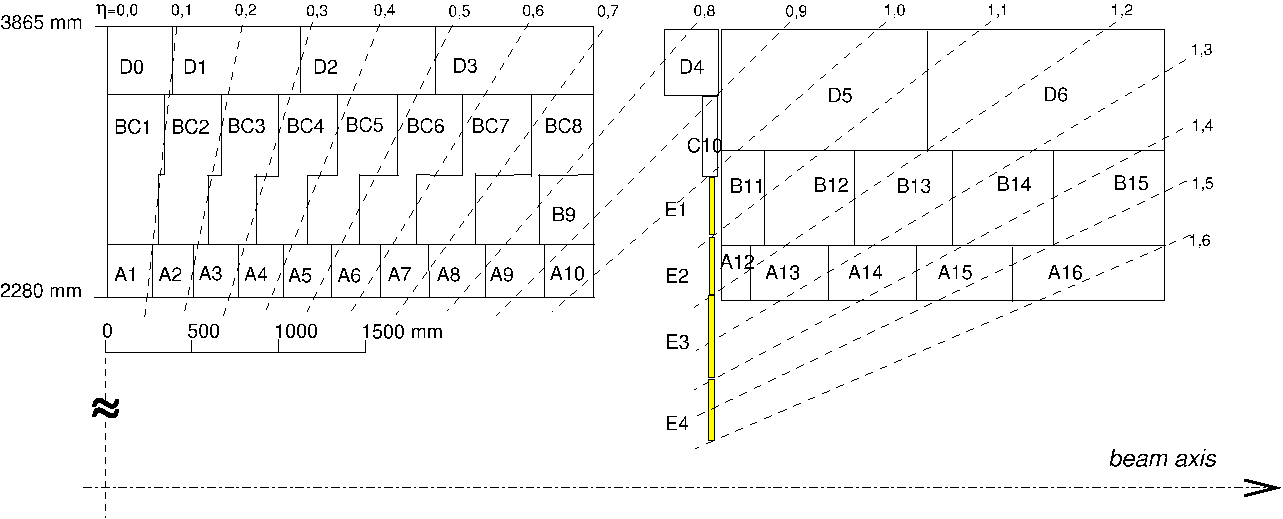
\includegraphics[width=\linewidth]{tile_cells}
    \caption{Schematic view of the TileCal scintillator structure~\cite{TileCalPub}.}
    \label{fig:tile_cells}
\end{figure}
%%% Local Variables:
%%% mode: latex
%%% TeX-master: "../search_for_DM_LED_with_ATLAS"
%%% End:
